\documentclass[14pt, a4paper]{extarticle}
\usepackage[margin = 1in]{geometry}
\usepackage{graphicx}
\usepackage{hyperref}
\hypersetup{
    colorlinks=true,
    linkcolor=black,     
    urlcolor=cyan,
}

\begin{document}

    % begin{cover-page}
    	\thispagestyle{empty}
    	\begin{center}
    		JSS Mahavidyapeetha \\JSS Science and Technology University, \\Mysore 570006
    		
    		\vspace{0.25in}
    		
\includegraphics[scale=1.25]{images/jssstulogo.jpg}
    		
    		\vspace{0.75in}
    		{\Large \textbf{Epidemic Simulation}}
    		
    		\paragraph{}
    		Project synopsis submitted in partial fulfillment of the curriculum prescribed for the Final Year Project for the award of the degree of
    		
    		\paragraph{}
    		\textbf {Bachelor of Engineering \\in \\Computer Science and Engineering \\By}
    
            \vspace{0.25in}
            \begin{table}[h!]
                \begin{center}
                    \begin{tabular}{|c|c|}
                    \hline
                    \textbf{USN} & \textbf{Name}\\
                    \hline
                    01JST17CS024 & Anuj Yadav \\
                    01JST17CS052 & Eeshaan Achar \\
                    01JST17CS080 & Manjunath Badakar \\
                    01JST17CS142 & Saurav Kumar \\
                    \hline
                    \end{tabular}
                \end{center}
            \end{table}
    
            \vspace{0.75in}
            Submitted to \\\textbf{Dr. H C Vijayalakshmi} \\Department of CS\&E, \\JSSSTU Mysore
        \end{center}
    % end{cover-page}
    
    \newpage
    \thispagestyle{empty}
    \section*{Acknowledgement}
        This project has been made possible by the kind support of many individuals such as our friends and families, and organizations such as our university. We wish to extend our sincere gratitude to all of them. We would also like to express gratitude to our mentor Dr. H C Vijayalakshmi, as without her guidance in the past as well as in the coming days, this project would not have been feasible. Lastly, we would like to thank our fellow teammates for their time and efforts, without which this project would not have seen the light of the day.

	\newpage
	\thispagestyle{empty}
	\tableofcontents

	\newpage
	\pagenumbering{arabic}
	\section{Problem Statement and Hypothesis}
	    \paragraph{The Problem:} An Epidemic is an outbreak of a disease that spreads rapidly and widely. Epidemics such as the Bubonic Plague, Avian flu, H5N1 influenza, H1N1 swine flu, SARS etc. have disturbed human lives for centuries causing massive number of deaths and illnesses among people and animals. As the number of urbanized and mobile population has increased, the possibility of a worldwide pandemic has grown too. The coronavirus pandemic is a testament to the same. 

        \paragraph{Necessity of a Solution:} Understanding the ways in which diseases propagate has several benefits such as improving healthcare systems, increasing life spans, and reducing the impact of biological warfare. Thus, it is very important for governmental authorities and healthcare agencies to understand how diseases spread and how to limit this spread by selecting the best mitigation and social strategies. Examples of mitigation strategies include vaccination, antiviral treatment, and household prophylaxis. Social distancing strategies include school closure, quarantine, and isolation.

        \paragraph{The proposed Solution:} In this research, we propose to simulate the spread of a disease on a small population and record the results. Based on the disease, and the various measures taken to limit its spread, we would like to accordingly tweak the parameters and observe the variations in the result. We would also like to summarizes the main technical challenges in this field. Historically, epidemics have been modelled mathematically to understand their dynamics. These models can vary from a few simple equations to complex systems that need to be simulated on supercomputers. The latest advances in high performance computing and computational network science can help epidemiologists develop large-scale high fidelity models of the epidemic spread. These models can help guide public health officials and policy makers in taking appropriate decisions to prevent and control the epidemics.

	\newpage
	\section{Objectives and Scopes}
	    \paragraph{} Objective is the aim or the final result we wish to achieve by completing a certain process. The scope of a process defines the limitations that we have to face while completing a process. For a successive process, the objectives have to be achieved within the scope.
	    
	    \subsection{Objectives}
    	    \begin{itemize}
    	        \item Simulate the spread of a disease on a social network model and to obtain information about that disease such as it's rate of spreading, the rate of recovery of victims, the fatality and mortality rates etc.
    	        
    	        \item Understand and appreciate the effect of various proposed safety measures such as social distancing, hand washing etc. amidst the prevailing coronavirus pandemic, through the simulation of the same.
    	        
                \item Understanding the various social network models available in the literature, along with their working and relevance.
                
                \item Appreciating the contributions of various research scholars through their published work, and also propose any improvements if found and feasible.
    	    \end{itemize}
	    
	    \subsection{Scopes}
    	    \begin{itemize}
    	        \item The simulation will consist of a small sample of population, expected to be around 1000 nodes. This is unlike the real world which consists of over 7 billion humans beings and trillions of other creatures.
    	        
    	        \item Unlike the real world where the behaviour of people vastly differs from each other and is highly unpredictable, the nodes in our simulated world will have a much more defined behaviour.
    	        
    	        \item An epidemic will have varied statistics across varying geography. In this simulation however, these statistics will be fed as parameters and will be constant for the entire population.
    	    \end{itemize}
	
	\newpage
	\section{Literature Review}
	    \paragraph{} The epidemic progression of COVID-19 has received increased attention from the research community since its outbreak in late 2019. The importance of understanding the virus transmission dynamics, and further predicting the epidemic curve for public policy healthcare control measures, has prompted multiple modeling efforts to control the outbreak and raised multiple questions around the same. Existing contributions in the epidemiological modeling of COVID-19 include different types of models, such as statistical models, mathematical models, network-based models, and phenomenological models. Due to their conceptual and mathematical simplicity, mathematical models, especially SIR compartmental models, have long been popular in modeling epidemic dynamics.
	    
	    \subsection{Simulation of the COVID-19 epidemic on the social network of Slovenia}
	        \paragraph{} In this research paper by Aleksandar Gavrić and Ziga Zaplotnik, they have developed a virus transmission model on the simplified social network of Slovenia with 2 million nodes organized into home/care center clusters. A detailed disease progression model is coupled with the virus transmission model. In this study, they evaluated the contribution of the virus transmission uncertainty (e.g. reproduction number and its derivatives), network and initial condition uncertainty and uncertainty of the disease progress model to the total uncertainty of the epidemic forecast. They found that in the uncontrolled epidemic, the intrinsic uncertainty mostly originates from the uncertainty of the virus transmission, while the randomness of the social network has only minor impact of the final size of the epidemic. The latter is in line with a study, where the social network was constructed based on extensive contact survey data, and which reported only minor impact of reshaping the network structure or removing the variance of connection weights on the final size of the epidemic. On the opposite, in the controlled epidemic with low infected population, the randomness of the social network becomes the major source of forecast uncertainty. They also showed that the uncertainty of the forecast and the associated risk is extremely asymmetric (roughly symmetric on a logarithmic axis) with long exponential tails.
	
	    \subsection{A Social Network Model of the COVID-19 Pandemic}
	        \paragraph{} The social network model developed by Pei Jun Zhao, Harvard T.H. Chan School of Public Health, provides a conceptual framework to analyze the COVID-19 pandemic on the level of individuals, that can be used to predict the influence of collective social behavior on overall pandemic trajectories. It shows the importance of social distancing, and the message that to contain the epidemic, every member of the public plays a crucial part in breaking the chain of transmission. The social network model of COVID-19 transmission is expandable and extendable. This paper provided a simplified version using population averages for parameters.
	
	\newpage
	\section{Research Methodology}
	    \paragraph{} Research can be defined as a systematic process of collecting data and logically analysing this data for a given purpose. Research methods constitute ways in which one collects and analyses the data to acquire knowledge reliably and validly. This section describes the methodology and procedures applied to achieve the objective of this research.

        \paragraph{} The primary goal of this research is to simulate an epidemic and analyse how it spreads on a small sample of population. We would also like to understand the effects of various real life factors such as infection probability, recovery rate, isolation, travel frequency, social distancing measures etc. on this simulation, which can provide a better intuition in understanding the epidemic on a larger scale.
        
        \paragraph{} The research will be carried out in two stages. The first stage will be to simulate the spread of the epidemic over the population sample. Python along with its NetworkX package will be used for the purpose. The second stage will be to tweak the various parameters mentioned before, and document the variations in the results obtained. The two stages will be repeated as necessary, as per the incremental software model.
        
        \paragraph{} To build a simulation which is in proximity to the real world we will be using a model called the SIR model which was introduced by Kermack and McKendrick. In this model we will fractionate our population or sample into 3 types of categories namely Susceptible(S), Infected(I) and Removed(R).
        
        \begin{itemize}
            \item Susceptible - This group in the population are the ones who are currently not infected with the disease but can acquire it if they are inside the infectious radius of an infected person for a certain amount of time.
            
            \item Infected - This class of people are the ones who have acquired the disease in the population.
            
            \item Removed - This is the group of population who have either recovered from the disease after a specified period of time or have died due the disease.
        \end{itemize}
        
        \begin{center}
            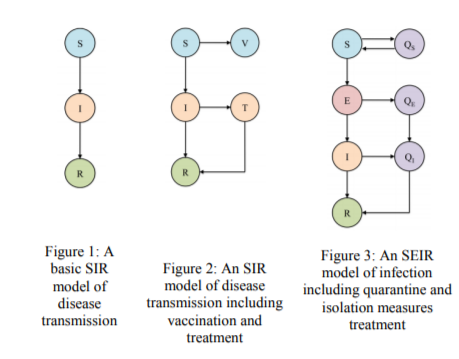
\includegraphics[scale=1.25]{images/sir_diag.png}
        \end{center}
        
        \paragraph{} An extension to the SIR model which includes two biomedical interventions is shown in Figure 2. A susceptible individual (S) can be vaccinated (V), and an infected individual (I) can be treated with antiviral drugs (T) and then moved to the recovered state (S). Figure 3 shows the Susceptible-Exposed-Infectious-Recovered (SEIR) model with an extension that includes two behavioral interventions which are quarantine (QS) and isolation (QI).
	
	\newpage
	\section{References}
	    \paragraph{} The following articles, research papers and videos greatly influenced the project by providing all the necessary insights needed to get started.
    	
        \begin{itemize}
            \item Simulating an epidemic by 3Blue1Brown. \href{https://www.youtube.com/watch?v=gxAaO2rsdIs}{See here}.
            
            \item Why outbreaks like coronavirus spread exponentially, and how to “flatten the curve” by Harry Stevens. \href{https://www.washingtonpost.com/graphics/2020/world/corona-simulator/}{See here}.
            
            \item Outbreak by Kevin Simler. \href{https://meltingasphalt.com/interactive/outbreak/}{See here}.
            
            \item Exponential growth and epidemics by 3Blue1Brown. \href{https://www.youtube.com/watch?v=Kas0tIxDvrg}{See here}.
            
            \item Simulation of the COVID-19 pandemic on the social network of Slovenia by Žiga Zaplotnik, Aleksandar Gavrić and Luka Medic. \href{https://journals.plos.org/plosone/article?id=10.1371/journal.pone.0238090}{See here}.
            
            \item A Social Network Model of the COVID-19 Pandemic by Pei Jun Zhao. \href{https://www.medrxiv.org/content/10.1101/2020.03.23.20041798v1.full-text}{See here}.
            
            \item Social Networks by IITM. \href{https://www.youtube.com/playlist?list=PLyqSpQzTE6M8CLBcLnq-f3vHRH-klC39L}{See here}.
            
            \item Effect of delay in diagnosis on transmission of COVID-19 by Xinmiao Rong, Liu Yang, Huidi Chu and Meng Fan. \href{http://www.aimspress.com/article/10.3934/mbe.2020149}{See here}.
        \end{itemize}
	
\end{document}